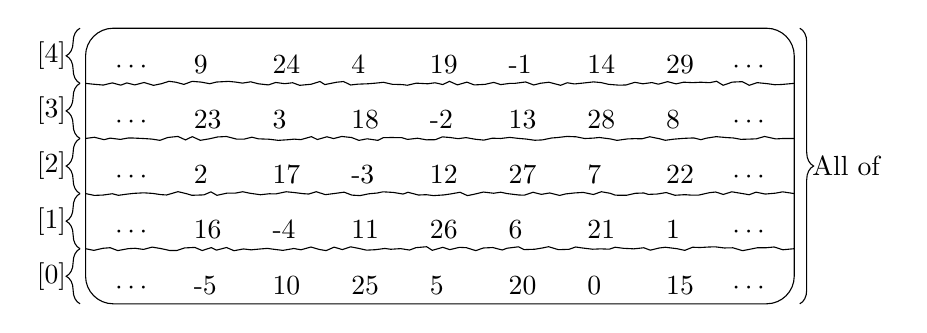
\begin{tikzpicture}
% Set and set contents
    \draw[rounded corners=10pt] (-1,0) rectangle (8,3.5);
    \foreach \y in {0.7,1.4,...,2.8}{
        \draw[decorate,decoration={random steps,segment length=3pt,amplitude=0.75pt}] (-1,\y) -- (8,\y);
    };
    \foreach \x in {0,...,6}{
        \foreach \y in {-5,2,9,16,23}{
            \pgfmathparse{int(\y+\x)}\let\y=\pgfmathresult;
            \pgfmathparse{int(Mod(\y,5))}\let\mult=\pgfmathresult;
            \node[anchor=south west] at (\x+0.25,0.7*\mult){\y};
        }
    }
% Labels
    \draw[decorate,decoration={brace,amplitude=5pt,raise=2pt}] (8,3.5) -- (8,0) 
        node[pos=0.5,right,anchor=west,xshift=3pt]{All of \(\bbZ\)};
    \foreach \y in {0,...,4}{
        \draw[decorate,decoration={brace,amplitude=5pt,raise=2pt}] (-1,0.7*\y) -- ++(0,0.7) 
            node[pos=0.5,left,anchor=east,xshift=-3.5pt]{\([\y]\)};
        \node[anchor=south west] at (-0.75,0.7*\y) {\(\cdots\)};
        \node[anchor=south east] at (7.75,0.7*\y) {\(\cdots\)};
    };
\end{tikzpicture}